\chapter{Up-scaling experimentation in cell biology}
\paragraph*{} Existing microscope software requires a human operator to scan the sample visually, and identify regions of interest for imaging sample objects. However, it is difficult for the human user to manually comb through the sample to find fields of interest. Combing the sample for objects can also expose it to large amount of light, which can cause photobleaching of the flurophores or create destructive phototoxicity artifacts \cite{scherf2015smart}. Besides, the execution plan of the microscope is rigid, and the user must take care to configure the plan correctly, and there is no scope for error correction during an acquisition without discarding data or timepoints. Feedback of the validity of the experimental data is often obtained in the image analysis stage of the microscopy experiment, by which time it is too late to influence the experiment, take corrective measures such as reimaging the sample. Such problems are fundamental to microscopy technology, and are faced by several others in fields such as super-resolution microscopy \cite{D1SC05506B}. We developed full-stack microscopy, which combines acquisition with analysis, which is often considered separate steps of an imaging experimental workflow. This allows us to get a direct feedback of experimental quality during the course of imaging. In our case, we wanted to maximize the sample size of common DDR experiments, while minimizing light exposure to the sample prior to data acquisition.


\section{Overview of existing technology}
\paragraph*{}The software systems of commonly available widefield systems can be characterized as open loop systems. The user configures the microscope for a specific mode of operation by choosing appropriate device parameters manually. Some of these parameters are position of stage, Z drive, mirrors, shutter, detector exposure, detector gain, choice of objective, etc. Many of these parameters are optimally set to attain the best image possible by the system in order to perform further downstream analysis. The best image is often characterized as an image that has one or many or a part-of an object of interest (such as cells, tissues, crystals, etc), is well focused, well-illuminated, with good contrast, and without any over-exposed pixels, which are niquest sampled.

Some of these considerations for best image translates to the user having to manually scan the sample, which can have different forms, such as a confocal dish, slide, or a multi-well plate, in search of fields of interest. In the case of a confocal dish, one has to ensure that the field of interest is not set in the periphery of the coverslip area, where light will move through glass and plastic, reducing the quality of the image. Other considerations of the field might be determined by the object of interest under observation. One might want to image only cells transfected with a certain plasmid expressing one or more fluorescent proteins. Or one might be interested in imaging cells of certain cell cycle stage, such as mitotic or s-phase cells. In such scenarios, to identify fields of interest is a task of human persistance. The more effort one can spend in identifying fields of interest, one casts a wider net of observation on their objects of interest, therefore increasing the throughput of the experiment.

The establishment of fields of interest by manual inspection translates to a list of stage coordinates, with which the microscope executes an imaging sequence, resulting in the production of data. Existing commercial software present this model which can be characterized as an open loop, where the chain of execution is linear, and there are no feedback in the operation of the system.

The user takes the data from the microscope software, and often starts a separate control sequence for image analysis, which results in quantifiable information that can be graphically represented to support the initial hypothesis. The analysis maybe manually done with ImageJ or automated partially or fully with macros or using other programming languages capable of image processing and statistical analysis, such as Python, or Matlab. This disconnect between the control sequences of imaging and analysis creates a gap in the experimental process that has to be bridged by the human user. In case the analysis reveals problems in imaging (such as focus drift, xy-drift, over or under exposed image, or insufficient sample size), there is no way for the analysis control sequence to make adjustments to the acquisition control sequence to compensate for low-quality data. Even if such compensations are done manually, it is time-consuming and might not yield the desired experimental conditions for the user. It is analogous to the era of satellite imaging (before digital camera) which used photographic films to image the Earth, and the film had to be later ejected into the atmosphere, captured, and developed in a lab, and often the pictures were out of focus, or had cloud cover over their area of interest, marking for poor returns from a costly mission. Experiments with biological sample could be time-bound, and would have to be verified for quality at every acquisition step. Sample undergoing treatment conditions, or samples such as primary tissues are time-sensitive and cannot be imaged again once a timepoint has elapsed. Corrections would have to be performed online in case of any imaging failure. However, with the disconnect between acquisition and analysis, it is not often possible to make such corrections without manual inspection at the time of acquisition, making this a high-effort endeavour.


\section{Microscope software from scratch}
In order to combine the acquisition and analysis of microscope software, and to build on top of that, one would have to write a microscope control software from scratch. In a control system point of view, a microscope can be abstracted as a combination of motors and detectors. Motors are devices such as the filter wheel, objective turret, temperature control unit, condensor unit, etc. and detectors are the camera unit, or a quadrant photodiode that returns a reading of the sample. The challenge is to be able to communicate with these devices and be able to set and read state parameters of these motors programmatically. Such as, reading the current position configuration of the filter wheel, or setting the objective turret to new position. For any motor-like device, this can be abstracted as set and read functions.

Microscope software can be thought of as abstractions of increasing complexity that work on top of each other. At the most basic level, the microscope software should be able to send commands to the device, and receive responses. This is often known as the control layer, which facilitates control at the hardware level. In the other hand, the device receives the command signal from the user, executes it, and sends a response. This communication to the device is often facilitated through a serial communication protocol, which takes messages to and from the device through a physical medium, such as a cable with multiple pins, the two ends of which are attached to the motherboard of the control computer and the device that is to be controlled. In the computer end, there are device drivers, which organized for the specific device for the messages to be sent through the serial port, for the high level tasks that are to be accomplished for that device. For instance, there might be an exposure set command to set a certain exposure for the camera, or a snapshot command for taking a snapshot. At the device level, these might translate to a multitude of actions, which are abstracted away inside the device. The device acts as a message parsing hub, which receives messages, performs actions and replies with data.

With the control over the hardware with device drivers defined, it then becomes a matter of establishing connection with all the devices, and orchestrating the order in which the devices are asked to perform a certain task programmatically. 


\paragraph*{} Towards that, I utilized pymmcore, the python wrapper for micro-manager to get raw access to the control layer of the microscope hardware (Olympus IX83, Andor Zyla camera) \cite{edelstein2014advanced}. This enabled me to change the state of different motors, and read image data from the camera, therefore creating an acquisition pattern.

I integrated micro-manager control layer with bluesky, a spectroscopy based data acquisition framework, which gave me the necessary higher-level abstractions to define complex workflows, redundancies, error-checking and data management \cite{allan2019bluesky}.

\begin{figure}[H]
    {\hfill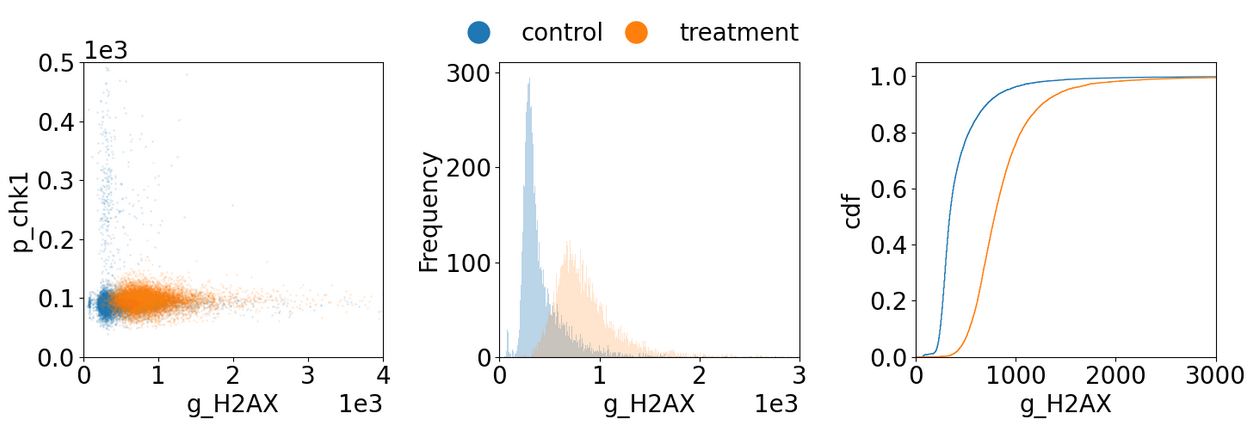
\includegraphics[clip, width=1\linewidth]{figures/ncs.png}\hspace*{\fill}}
    \caption{Automated immunofluorescence imaging against $\gamma$H2AX and phosphorylated Chk1 with a sample size of N=11000 for control and treatment each.}
    {\label{fig:ncs}}
\end{figure}

\paragraph*{} Using this tool, we pushed the limit of sample size for a damage response experiment based on immunofluorescence against $\gamma$H2AX and phosphorylated Chk1. We chemically induced damage, and imaged a total of 22000 cells, (11000 each for control and treated) with no human effort in imaging (Fig. \ref{fig:ncs}). This is far higher cell numbers than what is regularly done in microscopic investigations of DDR using everyday widefield microscopes. High Content microscopes can achieve such numbers, but we have now implemented this solution on a regular motorized widefield microscope, increasing the breadth of such investigations.

\begin{figure}[H]
    {\hfill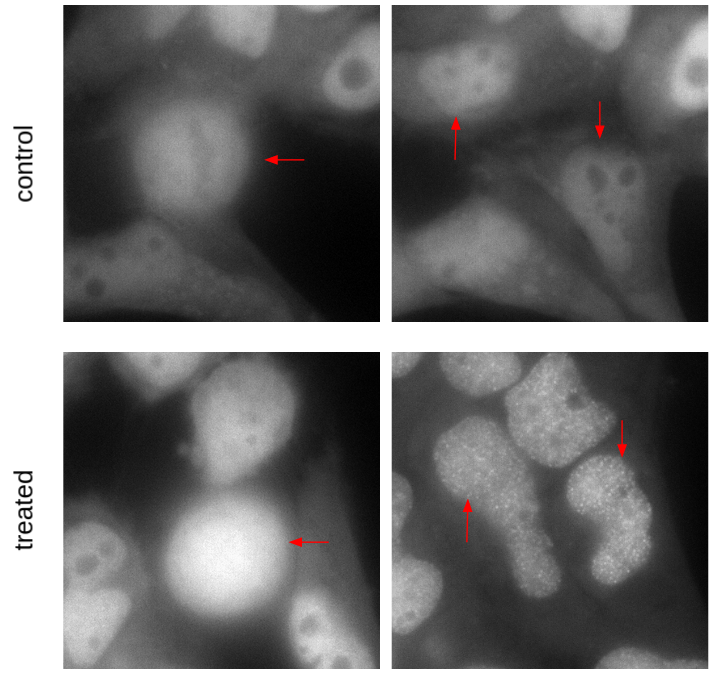
\includegraphics[clip, width=0.8\linewidth]{figures/g1.png}\hspace*{\fill}}
    \caption{G1 cells show punctated PCNA upon 4NQO damage. We followed mitotic cells (left) over time, until they divided into G1 cells. Treated G1 cells show punctated PCNA. The arrows are marking parent (left) and daughter cells (right)}
    {\label{fig:g1}}
\end{figure}

\paragraph*{} We further developed this tool to image live cells over high cell numbers to identify small subpopulations of interest. We imaged a large volume of HeLa cells expressing PCNA-chromobody, and induced damage with 4NQO. We observed that PCNA is punctated in non-S phase cells, indicating foci of repair. Furthermore, we also observed that damage foci are transferred to daughter G1 cells from a dividing mitotic cell (Fig. \ref{fig:g1}). This required us to acquire data over hundreds of cells in an asynchronous population. Potentially such studies can be done by chemically arresting cells in specific stages of the cell cycle and then releasing them. But such arrests themselves can alter measured responses, and there is value in performing studies in unperturbed asynchronous cultures.

\paragraph*{} In summary, we assembled a microscope acquisition software from scratch for hands-free high throughput data acqusition. We applied it to DDR and saw that we can push the sample size of traditional immunofluorescene experiments to N greater than 10,000 with no effort from the user. We increased throughput for live-cell imaging, and saw that PCNA foci form in bona fide G1 cells created right after a mitosis event.
